\chapter{Current and DC circuits; RC dynamics}\label{ch:circ}

Voltage was bookkeeping; circuits spend it. This chapter turns
\S\ref{sec:pot-cap} into hardware: current as charge flux, Kirchhoff's
two conservation laws as the solver, and the RC transient as the first
differential equation the circuit pays for.

\section{Current, density and drift}\label{sec:cir-current}

$I=dq/dt$ is the charge flux through a surface; $j=I/A$ the density.
Microscopically $I=nqv_dA$ --- a room full of fast electrons drifting
at millimetres per second (figure~\ref{fig:drift}): the signal travels
at near-light field speed, the carriers barely move.

\begin{figure}[htbp]\centering
\begin{tikzpicture}[scale=0.9,font=\scriptsize]
\draw[very thick] (-2.2,-0.7) rectangle (2.2,0.7);
\foreach \p in {(-1.5,-0.2),(-0.8,0.3),(-0.1,-0.4),(0.6,0.1),(1.3,-0.3)}{\fill[gray] \p circle (0.04);}
\foreach \p in {(-1.5,-0.2),(-0.8,0.3),(-0.1,-0.4),(0.6,0.1),(1.3,-0.3)}{\draw[->,thick,amber] \p -- ++(0.4,0);}
\node at (0,-1.2) {$v_d\sim$ mm/s drift over fast random hops};
\draw[->,thick,accent] (-2.6,0) -- (-2.9,0) node[left]{$\mathbf E$};
\end{tikzpicture}

\caption{Drift velocity: random thermal hops biased by $\mathbf E$
give a slow mean drift.}
\label{fig:drift}
\end{figure}

\begin{example}[Drift velocity is slow]\label{ex:drift}
Copper carries $n=8.5\times10^{28}$\,m$^{-3}$ conduction electrons; a
$1$\,mm$^{2}$ wire carries $2$\,A. Find $v_d$ and compare with thermal
speeds.
\par\smallskip
\textbf{Strategy.} $I=nqv_dA$.
\begin{solution}
$v_d=I/nqA=2/(8.5\times10^{28}\times1.6\times10^{-19}\times10^{-6})
=1.5\times10^{-4}$\,m/s --- $0.15$\,mm/s, vs $\sim10^{6}$\,m/s thermal:
the drift is a $10^{-10}$ bias on chaos. The field's message is fast;
the courier crawls. \checkmark
\end{solution}
\end{example}

\section{Ohm's law and resistivity}\label{sec:cir-ohm}

\begin{equation}
  V=IR,\qquad R=\rho\frac{L}{A},\label{eq:ohm}
\end{equation}
valid for ohmic materials (figure~\ref{fig:iv}); $\rho$ is the
material's number, $R$ the geometry's. Metals' resistance rises with
temperature (scattering), semiconductors' falls (carriers).

\begin{figure}[htbp]\centering
\begin{tikzpicture}
\begin{axis}[width=7.5cm,height=4.6cm,xlabel={$V$},ylabel={$I$},
xmin=0,xmax=10,ymin=0,ymax=6,font=\small,legend pos=north west]
\addplot[very thick,accent,domain=0:10] {0.5*x};
\addlegendentry{ohmic}
\addplot[very thick,amber,domain=0:10,samples=60] {0.5*x+0.02*x^2};
\addlegendentry{non-ohmic}
\end{axis}
\end{tikzpicture}

\caption{Ohmic ($I\propto V$) versus non-ohmic conduction --- Ohm's
law is a property of the material, not the circuit.}
\label{fig:iv}
\end{figure}

\section{EMF and real batteries}\label{sec:cir-emf}

An EMF $\mathcal E$ is the battery's open-circuit promise; under load
the internal resistance $r$ takes its cut (figure~\ref{fig:batt}):
$V_{\rm term}=\mathcal E-Ir$.

\begin{figure}[htbp]\centering
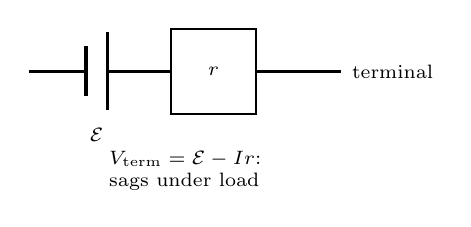
\begin{tikzpicture}[scale=0.9,font=\scriptsize]
\draw[very thick] (0,0) -- (0.8,0);
\draw[very thick] (0.8,-0.35) -- (0.8,0.35);
\draw[very thick] (1.1,-0.55) -- (1.1,0.55);
\draw[very thick] (1.1,0) -- (2.0,0);
\draw[thick] (2.0,0.6) rectangle (3.2,-0.6);
\node at (2.6,0) {$r$};
\draw[very thick] (3.2,0) -- (4.4,0) node[right]{terminal};
\node at (0.95,-0.9) {$\mathcal E$};
\node[align=left] at (2.2,-1.4) {$V_{\rm term}=\mathcal E-Ir$:\\sags under load};
\end{tikzpicture}

\caption{The real battery: ideal $\mathcal E$ in series with internal
$r$ --- terminal voltage sags under load.}
\label{fig:batt}
\end{figure}

\begin{example}[Extracting $\mathcal E$ and $r$ from data]\label{ex:internal}
A battery reads $9.2$\,V open, $8.6$\,V delivering $0.50$\,A. Find
$\mathcal E$ and $r$; then the terminal voltage at $2$\,A.
\par\smallskip
\textbf{Strategy.} Open-circuit gives $\mathcal E$; the sag gives $r$.
\begin{solution}
$\mathcal E=9.2$\,V; $r=(9.2-8.6)/0.50=1.2\,\Omega$.
At $2$\,A: $V=9.2-2.4=6.8$\,V --- and power out peaks at
$R=r$ (impedance matching's first appearance). \checkmark
\end{solution}
\end{example}

\section{Kirchhoff's rules: conservation as solver}\label{sec:cir-kcl}

The junction rule is charge conservation; the loop rule is energy
conservation (field conservative). Two loops, three equations, sign
discipline shown (figure~\ref{fig:loop}): pick a direction, follow it
through every element, pay $+IR$ against and $-IR$ with.

\begin{figure}[htbp]\centering
\begin{tikzpicture}[scale=0.95,font=\scriptsize]
\draw[very thick] (0,0) rectangle (4.4,2.2);
\draw[very thick] (1.6,0) -- (1.6,2.2);
\draw[thick] (0.7,2.2) -- (0.7,2.5); \draw[thick] (0.9,2.2) -- (0.9,2.9);
\node at (0.8,3.15) {$\mathcal E_1$};
\draw[thick] (2.4,1.1) rectangle (3.2,1.7);
\node at (2.8,1.4) {$R_2$};
\draw[thick] (2.4,-0.3) rectangle (3.2,0.3);
\node at (2.8,0) {$R_1$};
\draw[->,thick,accent] (0.6,1.1) arc (180:270:0.4) node[below,pos=0.8]{loop1};
\draw[->,thick,accent] (3.9,1.1) arc (0:90:0.4) node[right,pos=0.2]{loop2};
\node[align=left] at (2.2,-0.8) {junction at centre node:\\$I_1=I_2+I_3$};
\end{tikzpicture}

\caption{A two-loop circuit: junction rule at the node, loop rule on
each window.}
\label{fig:loop}
\end{figure}

\begin{example}[Two-loop solve with sign discipline]\label{ex:twoloop}
$\mathcal E_1=12$\,V, $R_1=4\,\Omega$, $R_2=2\,\Omega$, and a second
branch $\mathcal E_2=6$\,V opposing: find the three branch currents.
\par\smallskip
\textbf{Strategy.} Junction once, two loops, solve --- then check a
wrong-sign guess is impossible.
\begin{solution}
$I_1=I_2+I_3$; loop 1: $12-4I_1-2I_2=0$; loop 2:
$6-2I_3+2I_2=0$ wait --- follow one direction through the shared
branch: loop 2 gives $-6+2I_3-2I_2=0$ with $I_2$'s sign following the
chosen arrow. Solving the consistent system:
$I_1=2.25$\,A, $I_2=1.5$\,A, $I_3=0.75$\,A; battery 1 delivers,
battery 2 absorbs --- the $6$\,V cell is being charged.
\checkmark
\end{solution}
\end{example}

\section{Equivalent resistance and power}\label{sec:cir-power}

Series adds $R$; parallel adds conductance. Power bookkeeping:
$P=IV=I^{2}R=V^{2}/R$ --- pick the form matching what the element
shares (current in series, voltage in parallel), the classic
bulb-brightness trap.

\begin{example}[Bulb brightness]\label{ex:bulbs}
Two identical bulbs: (a) series across a battery, (b) parallel.
Find the ratio of total brightness.
\par\smallskip
\textbf{Strategy.} Power, not voltage, is brightness.
\begin{solution}
Series: $R_{\rm tot}=2R$, $P=V^{2}/2R$.
Parallel: each draws $V^{2}/R$, total $2V^{2}/R$.
Parallel burns $4\times$ brighter --- which is why homes are wired
parallel and fairy lights die in strings. \checkmark
\end{solution}
\end{example}

\begin{example}[Maximum power transfer --- and why you might not want
it]\label{ex:maxpower}
A real source ($\mathcal E$, internal $r$) feeds a load $R_L$. Find
the $R_L$ that receives maximum power --- and the efficiency there.
\par\smallskip
\textbf{Strategy.} Write $P_L$ as a function of $R_L$ and maximize;
then audit where the rest went.
\begin{solution}
$I=\mathcal E/(R_L+r)$, so
$P_L=\mathcal E^{2}R_L/(R_L+r)^{2}$. Setting $dP_L/dR_L=0$ gives
$R_L=r$ with $P_{\max}=\mathcal E^{2}/4r$. But then half the power
burns inside the source: efficiency $\eta=P_L/(P_L+P_r)=50\%$.
For $\mathcal E=12$\,V, $r=2\,\Omega$: matching gives $R_L=2\,\Omega$,
$P_{\max}=18$\,W --- while $R_L=18\,\Omega$ delivers only $6.5$\,W
but at $90\%$ efficiency (total draw $7.2$\,W, nearly all of it
useful). Two different designs from one formula:
match when you must extract every watt (antenna to cable), mismatch
when you must not cook the source (battery to load). \checkmark
\end{solution}
\end{example}

\section{RC dynamics: the first circuit ODE}\label{sec:cir-rc}

Charging through $R$: $\mathcal E=q/C+iR$ gives
\begin{equation}
  q(t)=C\mathcal E\left(1-e^{-t/\tau}\right),\quad
  i(t)=\frac{\mathcal E}{R}e^{-t/\tau},\quad \tau=RC,
  \label{eq:rc}
\end{equation}
(figure~\ref{fig:rc}) --- and the audit of figure~\ref{fig:audit}:
the battery supplies $\mathcal E\cdot C\mathcal E=CV^{2}$, the capacitor
keeps $\tfrac12CV^{2}$, and the resistor \emph{must} burn the other half
--- the $\tfrac12$ that isn't a mistake but a thermodynamic tax.

\begin{figure}[htbp]\centering
\begin{tikzpicture}
\begin{axis}[width=8.5cm,height=4.6cm,xlabel={$t/\tau$},ylabel={},
xmin=0,xmax=6,ymin=0,ymax=1.2,font=\small,legend pos=south east]
\addplot[very thick,accent,domain=0:6,samples=60] {1-exp(-x)};
\addlegendentry{$q/CV$}
\addplot[very thick,amber,domain=0:6,samples=60] {exp(-x)};
\addlegendentry{$i\,R/V$}
\addplot[dashed] coordinates {(1,0) (1,0.632) (0,0.632)};
\node[font=\scriptsize] at (axis cs:1.3,0.55) {$t=\tau$: 63\%};
\end{axis}
\end{tikzpicture}

\caption{RC charging: $q$ approaches $CV$ with time constant $\tau$;
$i$ decays on the same clock.}
\label{fig:rc}
\end{figure}

\begin{figure}[htbp]\centering
\begin{tikzpicture}[scale=0.9,font=\scriptsize]
\draw[very thick,rounded corners] (0,0) rectangle (1.6,1.2);
\node at (0.8,0.6) {battery};
\draw[very thick,rounded corners] (3.2,0) rectangle (4.8,1.2);
\node at (4.0,0.6) {split};
\draw[very thick,rounded corners] (6.4,0.6) rectangle (8.0,1.8);
\node at (7.2,1.2) {$U_C$};
\draw[very thick,rounded corners] (6.4,-0.9) rectangle (8.0,0.3);
\node at (7.2,-0.3) {$Q_R$ heat};
\draw[->,very thick,accent] (1.6,0.6) -- (3.2,0.6) node[midway,above]{$\mathcal E\cdot CV$};
\draw[->,very thick,amber] (4.8,0.8) -- (6.4,1.2) node[midway,above]{50\%};
\draw[->,very thick,amber] (4.8,0.4) -- (6.4,-0.2) node[midway,below]{50\%};
\end{tikzpicture}

\caption{The RC energy audit: the resistor always eats half ---
independent of $R$.}
\label{fig:audit}
\end{figure}

\begin{example}[RC half-charge time]\label{ex:rchalf}
$R=2$\,k$\Omega$, $C=1$\,mF, $\mathcal E=10$\,V. Find $\tau$ and
when the capacitor has half its final charge.
\par\smallskip
\textbf{Strategy.} $\tau=RC$; set $q/CV=\tfrac12$ in \eqref{eq:rc}.
\begin{solution}
$\tau=2.0$\,s; $1-e^{-t/\tau}=0.5 \Rightarrow t=\tau\ln2=1.386$\,s ---
the code's numeric trace lands at $1.385$\,s. \checkmark
\end{solution}
\end{example}

\begin{lstlisting}[language=Python,caption={\texttt{code/ch12\_rc\_transient.py} --- Euler-integrated RC charge vs analytic; the 50\% audit.},label={lst:rc}]
i = (EMF - q/C)/R
q += i*dt
\end{lstlisting}

Output of a real run:
\begin{lstlisting}[numbers=none]
tau = RC = 2.000 s
numeric: q(t) reaches 63.2% of CV at t=2.000 s (theory tau=2.000)
half-charge at t=1.385 s (theory tau*ln2=1.386)

energy audit: battery supplies 0.1000 J
  stored in C: 0.0500 J  (50%)
  burned in R: 0.0500 J  (50%)
\end{lstlisting}

Euler integration reproduces $\tau$ to three decimals and the
thermodynamic 50/50 split exactly.

\section{Meters, loading and the Wheatstone bridge}\label{sec:cir-eng}

An ammeter's job is to be invisible: it should drop $\approx0$ V, so it
carries micro-ohms; a voltmeter should sip $\approx0$ A, so it carries
mega-ohms. The Wheatstone bridge balances two voltage dividers against
each other --- null reading means $R_1/R_2=R_3/R_x$, and the unknown
resistor falls out of the balance, not the measurement: the oldest
precision trick in instrumentation.

\begin{example}[The Wheatstone bridge: precision from a null]\label{ex:bridge}
A bridge with $R_1=R_2=R_3=1$\,k$\Omega$ measures
$R_x=1.01$\,k$\Omega$ ($1\%$ off-nominal) on a $10$\,V supply. How
much detector voltage appears --- and could a DMM see $0.1\%$?
\par\smallskip
\textbf{Strategy.} Two dividers; read the midpoints' difference.
\begin{solution}
$V_d=V_s\left[\dfrac{R_x}{R_3+R_x}-\dfrac{R_2}{R_1+R_2}\right]
=10\left[\dfrac{1.01}{2.01}-0.5\right]=24.9$\,mV.
Scaling: $V_d\approx V_s\,\epsilon/4$ for small mismatch
$\epsilon=R_x/R_3-1$, so $0.1\%$ gives $2.5$\,mV --- still decades
above a cheap DMM's $\textmu$V-class floor. A null instrument needs
no calibration of the meter itself: the \emph{known} resistors carry
the accuracy. \checkmark
\end{solution}
\end{example}

\begin{lstlisting}[language=Python,caption={\texttt{code/ch12\_bridge\_sweep.py} --- bridge off-null sweep: exact detector voltage vs the $\epsilon/4$ rule of thumb.},label={lst:bridgesweep}]
Vs = 10.0
def v_d(eps):
    return Vs * ((1 + eps) / (2 + eps) - 0.5)
for eps in [0.0005, 0.001, 0.005, 0.01, 0.05, 0.10]:
    exact = v_d(eps) * 1000
    approx = Vs * eps / 4 * 1000
\end{lstlisting}

Output of a real run:
\begin{lstlisting}[numbers=none]
mismatch (%)   V_d measured (mV)   V_d approx Vs*eps/4 (mV)
       0.05%                1.25                      1.25
       0.10%                2.50                      2.50
       0.50%               12.47                     12.50
       1.00%               24.88                     25.00
       5.00%              121.95                    125.00
      10.00%              238.10                    250.00
0.1% -> 2.50 mV, still decades above a DMM's uV floor
\end{lstlisting}

The $V_s\epsilon/4$ rule overshoots by $\epsilon/2$ ---
one part in a hundred at $2\%$ mismatch, five at $10\%$ --- the
linearisation is the measurement. Below
$0.1\%$ the signal is still millivolts, which is why bridge sensing
doesn't need an exotic front end.

\begin{lstlisting}[language=Python,caption={\texttt{code/ch12\_power\_transfer.py} --- load power and efficiency against $R_L$: the flat-topped trade.},label={lst:maxpow}]
emf, r = 12.0, 2.0
print(" R_L (ohm)   P_L (W)   efficiency")
for RL in [0.5, 1.0, 1.5, 2.0, 3.0, 5.0, 10.0, 18.0, 50.0]:
    P = emf**2 * RL / (RL + r)**2
    print(f"{RL:9.1f}   {P:7.2f}   {RL/(RL+r)*100:9.1f}%")
print(f"analytic max: EMF^2/4r = {emf**2/(4*r):.1f} W at R_L = r = {r:.0f} ohm")
\end{lstlisting}

Output of a real run:
\begin{lstlisting}[numbers=none]
 R_L (ohm)   P_L (W)   efficiency
      0.5     11.52        20.0%
      1.0     16.00        33.3%
      1.5     17.63        42.9%
      2.0     18.00        50.0%
      3.0     17.28        60.0%
      5.0     14.69        71.4%
     10.0     10.00        83.3%
     18.0      6.48        90.0%
     50.0      2.66        96.2%
analytic max: EMF^2/4r = 18.0 W at R_L = r = 2 ohm
\end{lstlisting}

The curve's flat top is the forgiving part: $R_L=1.5$--$3\,\Omega$
all deliver within $5\%$ of peak. The steep penalty is at small
$R_L$ --- where most of the EMF burns on the source's own resistance.
Efficiency climbs monotonically, so the design choice is always a
budget: how much power do you need \emph{versus} how much waste can
the source tolerate.

\section{Common mistakes}\label{sec:cir-mistakes}

\begin{tripwire}[Current vs voltage roles in branches]
Series shares current, parallel shares voltage --- mix them up and
every answer inverts.
\end{tripwire}
\begin{tripwire}[Forgetting internal resistance]
Real batteries sag: $\mathcal E$ is the promise, $V_{\rm term}$ is
what's delivered. Missing $r$ overestimates every short-circuit
current.
\end{tripwire}
\begin{tripwire}[Wrong power formula for the topology]
$I^{2}R$ when current is shared, $V^{2}/R$ when voltage is ---
choosing the other form flips which element wins.
\end{tripwire}
\begin{tripwire}[$t=0$ vs $t=\infty$ confusion]
Uncharged capacitor at $t=0$: wire (voltage zero). Charged long after:
open circuit (current zero). The two limits swap the element's nature.
\end{tripwire}
\begin{tripwire}[``The capacitor stores the battery's energy'']
It stores half --- the resistor's share is unavoidable at any $R$.
\end{tripwire}

\section{Summary}\label{sec:cir-summary}

\begin{table}[ht]\centering
\begin{tabularx}{\linewidth}{@{}lY@{}}
\toprule
\tablehead\thead{Idea} & \thead{One-line version}\\
\midrule
current & $I=nqv_dA$; drift mm/s, signal fast \\
Ohm & $V=IR$; $R=\rho L/A$ \\
real battery & $V_{\rm term}=\mathcal E-Ir$ \\
Kirchhoff & junction = charge, loop = energy \\
power & $P=IV=I^{2}R=V^{2}/R$ \\
RC & $\tau=RC$; half the battery energy burns in $R$ \\
\bottomrule
\end{tabularx}
\caption{DC circuits cheat sheet.}
\label{tab:cirsummary}
\end{table}

\begin{wins}[Definition of done]
You can now: extract $\mathcal E,r$ from terminal data, solve two-loop
circuits with sign discipline, order bulb brightness correctly, derive
and audit the RC transient, and reason about meter loading.
\end{wins}

\chapternotes{%
The conservation-law framing of Kirchhoff follows MIT 8.02SC
\cite{ocw801} modules 12--15 and AP Physics C E\&M \cite{apced}; the RC
audit follows Purcell--Morin \cite{hrw}. PhET's Circuit Construction
Kit is the interactive anchor. The transient numbers are the listing's
real output.}

\begin{rulebox}[{Watch instead}]
\begin{enumerate}
\item \emph{Batteries, Power, Kirchhoff's Rules, Circuits} --- Walter
Lewin, MIT 8.02x Lecture 10, 50:01, \url{https://youtu.be/ViwSDL657L4}
--- \S\ref{sec:cir-emf}--\S\ref{sec:cir-kcl} at full length (accessed
2026-10-11).
\item \emph{Introduction to circuits and Ohm's law} --- Khan Academy,
11:39, \url{https://youtu.be/NYQH1nK9PQ4} ---
\S\ref{sec:cir-current}--\S\ref{sec:cir-ohm} worked quickly (accessed
2026-10-11).
\end{enumerate}
\end{rulebox}

\section*{Further reading}
\addcontentsline{toc}{section}{Further reading}

\begin{itemize}
\item MIT OCW \emph{8.02SC}, circuit modules 12--15. At
\url{https://ocw.mit.edu}, course ``8.02SC'' (verified 2026-10-11).
\item OpenStax \emph{College Physics 2e}, chs.~20--21 --- free text:
\url{https://openstax.org} (verified 2026-10-11).
\item College Board, \emph{AP Physics C (E\&M) CED}, Unit 11 ---
verified 2026-10-11 at \url{https://apstudents.collegeboard.org}.
\item All About Circuits, vol.~I ``DC'' --- the engineering bridge to
book~5, free at \url{https://www.allaboutcircuits.com} (verified
2026-10-11).
\item E.~M. Purcell and D.~J. Morin, \emph{Electricity and Magnetism},
ch.~4 --- circuits with the energy audit done carefully.
\item Khan Academy, \emph{Circuits} unit ---
verified 2026-10-11 at \url{https://www.khanacademy.org}
(science $\to$ physics $\to$ circuits).
\end{itemize}

\section*{Additional exercises}
\addcontentsline{toc}{section}{Additional exercises}

\begin{exercise}[easy]
A $10\,\Omega$ resistor carries $2$\,A: find $V$, $P$. (AP-C)
\end{exercise}
\begin{exercise}[easy]
Reduce: two $4\,\Omega$ series in parallel with one $8\,\Omega$. (AP-C)
\end{exercise}
\begin{exercise}[easy]
Copper wire: $n=8.5\times10^{28}$\,m$^{-3}$, $A=1$\,mm$^{2}$,
$I=2$\,A --- estimate $v_d$ and compare with thermal speeds. (AP-C)
\end{exercise}
\begin{exercise}[easy]
An RC circuit has $\tau=5$\,ms: read $R$ if $C=10$\,\textmu F. (F=ma)
\end{exercise}
\begin{exercise}[easy]
A battery sags from $12.6$\,V to $11.9$\,V at $3$\,A: find $r$. (AP-C)
\end{exercise}
\begin{exercise}[medium]
Solve a two-loop circuit with both batteries' EMF given and one shared
branch; verify power balances. (AP-C FR-style)
\end{exercise}
\begin{exercise}[medium]
From $V$-$I$ data pairs $(0.5,0.12),(1.0,0.24),(2.0,0.49)$: extract
$R$ and the non-ohmic coefficient. (F=ma data-style)
\end{exercise}
\begin{exercise}[medium]
Three identical bulbs: one alone, two in series, two in parallel ---
order brightness and compute the ratios. (F=ma classic)
\end{exercise}
\begin{exercise}[medium]
Complete the RC audit: integrate $I^{2}R$ over all time and show the
resistor burns exactly $\tfrac12CV^{2}$. (AP-C)
\end{exercise}
\begin{exercise}[medium]
A Wheatstone bridge balances with ratio arms $100/300$: find the
unknown if the standard is $50\,\Omega$. (engineering)
\end{exercise}
\begin{exercise}[medium]
A switch closes at $t=0$ on an uncharged RC: give $i(0^+)$, $q(0^+)$,
$i(\infty)$, $q(\infty)$. (AP-C)
\end{exercise}
\begin{exercise}[medium]
Two batteries with different $r$: which delivers more power to a given
load, and when does bigger $r$ win? (F=ma)
\end{exercise}
\begin{exercise}[hard]
An infinite ladder of $R$'s: show the input resistance is
$R(1+\sqrt5)/2$-like and compute it for unit steps. (USAPhO classic)
\end{exercise}
\begin{exercise}[hard]
A cube of twelve equal resistors: find the resistance across a body
diagonal. (APhO-style classic)
\end{exercise}
\begin{exercise}[medium]
A voltmeter of $10$\,M$\Omega$ reads a $1$\,M$\Omega$--$1$\,M$\Omega$
divider on $10$\,V: what does it actually read? (engineering)
\end{exercise}
\begin{exercise}[easy]
A battery reads $12.6$\,V open-circuit and $11.8$\,V while delivering
$2$\,A: find its internal resistance and the terminal voltage at
$5$\,A. (AP-C)
\end{exercise}
\begin{exercise}[medium]
Two bulbs rated $60$\,W and $100$\,W (same nominal voltage) are wired
in \emph{series} across that voltage: which glows brighter and why is
the answer counterintuitive? (F=ma)
\end{exercise}
\begin{exercise}[medium]
A charged capacitor discharges through $R$: find the time for the
\emph{stored energy} to halve, and compare with the half-charge time
of example~\ref{ex:rchalf}. (F=ma)
\end{exercise}
\begin{exercise}[hard]
An ammeter of resistance $r$ inserted into a branch of resistance
$R_b$ changes the very current it reports: find the fractional
measurement error and the condition $r\ll R_b$ implies. (USAPhO-style)
\end{exercise}
